%!TEX encoding = UTF-8 Unicode
%!TEX root = ../lect-w05.tex

%%%

\ifkompendium\else

%\Subsection{Denna och nästa veckas uppgifter}
\begin{SlideExtra}{Övning: \texttt{classes}}
\begin{itemize}\SlideFontSmall
%!TEX encoding = UTF-8 Unicode

%!TEX root = ../compendium1.tex

\item Kunna deklarera klasser med klassparametrar.
\item Kunna skapa instanser med \code{new}.
\item Kunna ge argument vid instansiering.
\item Förstå innebörden av referensvariabler och värdet \code{null}.

\item Kunna använda nyckelordet \code{private} för att styra synlighet av attribut och konstruktorparametrar.

\item Förstå syftet med getters och setters.
\item Kunna förklara accessregler för kompanjonsobjekt.
\item Kunna skapa fabriksmetod i kompanjonsobjekt.
\item Känna till nyttan med en privat konstruktor.

%\item Kunna implementera en klass utifrån en specifikation.
\item Förstå skillnaden mellan referenslikhet och strukturlikhet.
\item Känna till skillnaden mellan \code{==} och \code{eq}, samt \code{!=} och \code{ne}.

\item Kunna förklara hur case-klasser hanterar instansiering.
\item Känna till hur case-klasser hanterar likhet.

\end{itemize}
\end{SlideExtra}

\begin{SlideExtra}{Lab \texttt{blockbattle} redovisas NÄSTA läsvecka 6}
  \begin{minipage}{0.42\textwidth}
        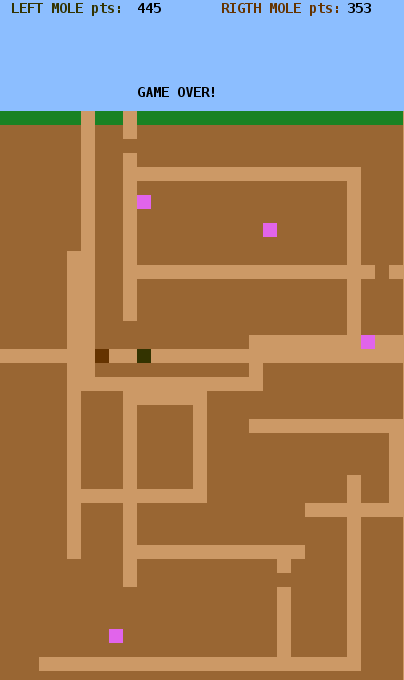
\includegraphics[height=0.8\textheight]{../img/blockbattle.png}
  \end{minipage}%
  \begin{minipage}{0.59\textwidth}
    \begin{itemize}\SlideFontTiny
      \item Ett arkadspel för TVÅ spelare.
      \item Nu med TVÅ blockmullvader!
      \item Går över TVÅ veckor:\\klasser (w05) \& matchning (w06).
      \item Programmet \code{blockbattle} är \Alert{mer omfattande} jmf m tidigare labbar.
      \item Läs igenom labben innan du gör övningarna.
      \item Kod från övningarna behövs till labben. 
      \item OBS! Labbtider är \Emph{schemalagda som vanligt} under läsvecka 5. Om du mot förmodan hinner redovisa redan denna vecka så ska du ändå närvara och t.ex. jobba med extrauppgifter. 
      \item Dra nytta av undervisningen så att du lär dig så mycket som möjligt!  
    \end{itemize}    
  \end{minipage}
\end{SlideExtra}
  
\fi
